\section{Apartment Building load profile}
\subsection{Heating profile}

The apartment building (Flatwoningen (overig) Gebouwd) build in the period 1965-1974 which represent 1.8 \texttt{\%} of the dutch housing stock \cite{VOORBEELD} (highest number in the flatwoningen category) will be selected. Houses in this category often have 2 to 4 rooms.The average gas consumption for this type of apartment (energy label C) is 829 $m^3$/year with the average usage area is 77 m2 and 2.8 people in the house. Label C has been selected because the focus of heat pump heating will be on the renovated house with good insulation. The property features are shown in Figure \ref{fig:features}.

\begin{figure}[H]
\centering
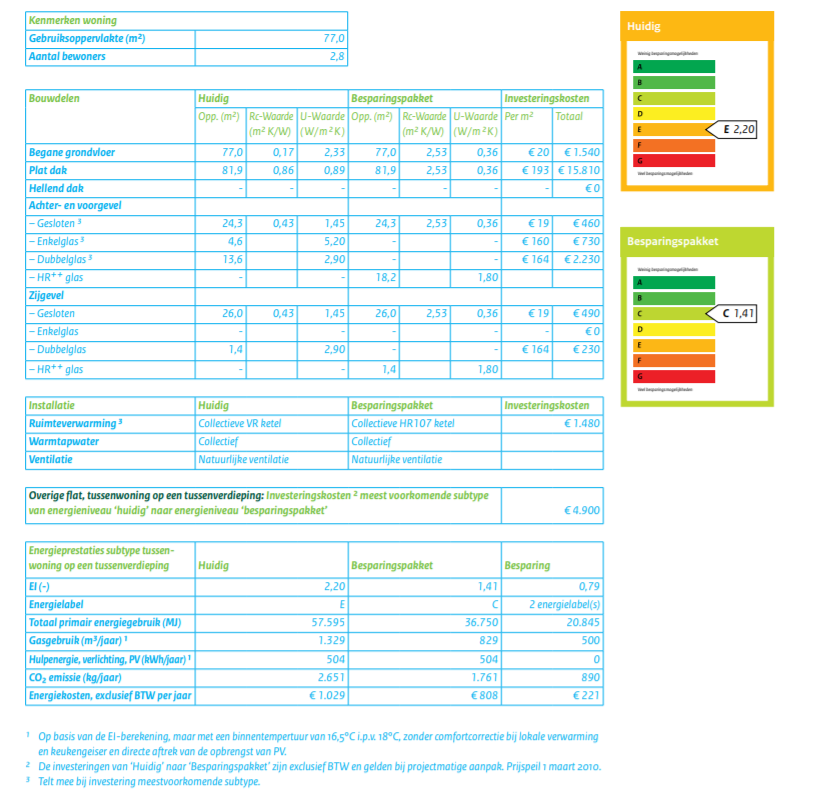
\includegraphics[width=1\columnwidth]{pictures/property features.png}
\caption[Short title]{property features \cite{VOORBEELD}.}
\label{fig:features}
\end{figure}

From \url{www.statista.com} (Figure \ref{fig:waterusage})one person use approximately 120 liters of water per day therein one third of the water is used for showering and bathing. The rest for washing, toilet and cooking.

\begin{figure}[H]
\centering
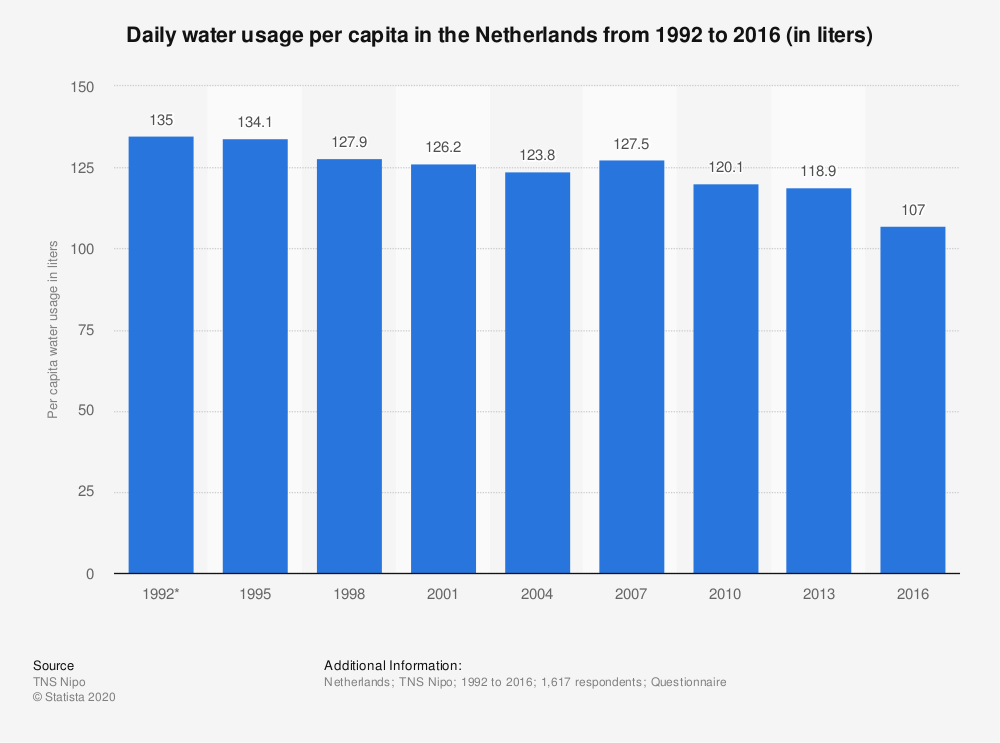
\includegraphics[width=1\columnwidth]{pictures/daily water usage.png}
\caption[Short title]{daily water usage by capital.}
\label{fig:waterusage}
\end{figure}


% If one person use around 60 liters of hot tap water at 40 degree per day. The energy use by one person can be calculated:

% \begin{equation}
% Q = m.c.\Delta T
% \end{equation}
% \\
% 60 liters $\approx$ 60 kg of water.\\
% c = 4.19 kj/kg.K specific heat capacity of water.\\
% $\Delta$T: temperature different: 40 - 10 = 30 $^o$C.\\ 
% \\
% At the results one person will consume 2.095kwh per day for hot tap water. 2.8 people will consume 5.866 kwh per day.\\
According to "VERORDENING (EU) Nr. 814/2013 VAN DE COMMISSIE van 2 augustus 2013" \cite{VERORDENING}. The hot water capacity M profile (will be discussed in next chapter) has a sum of energy use for tap water per day 5,845 kwh.

\begin{figure}[H]
\centering
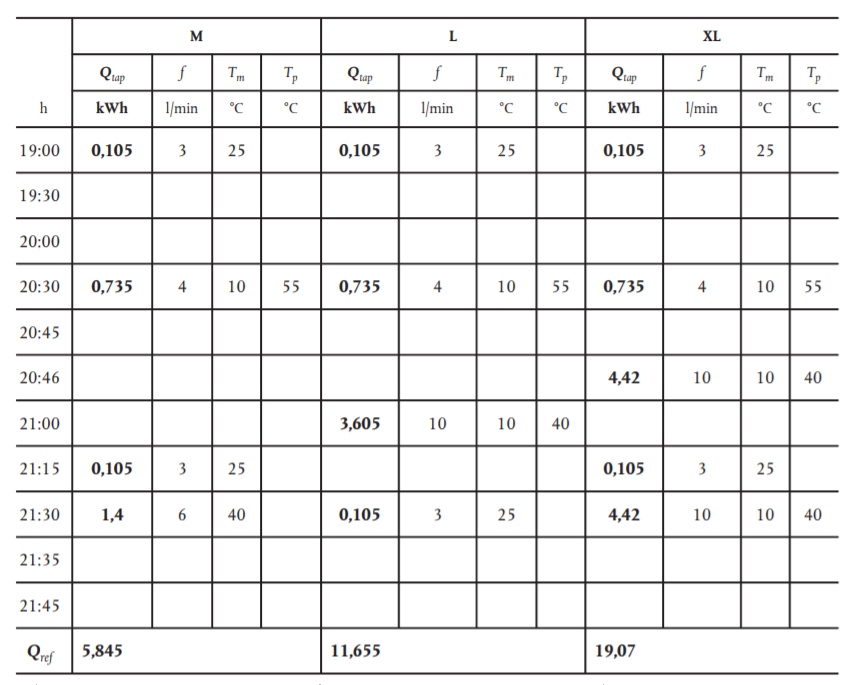
\includegraphics[width=1\columnwidth]{pictures/hot tap water.png}
\caption[Short title]{Example hot tap water profile.}
\label{fig:htwp}
\end{figure}


% \begin{figure}[H]
% \centering
% 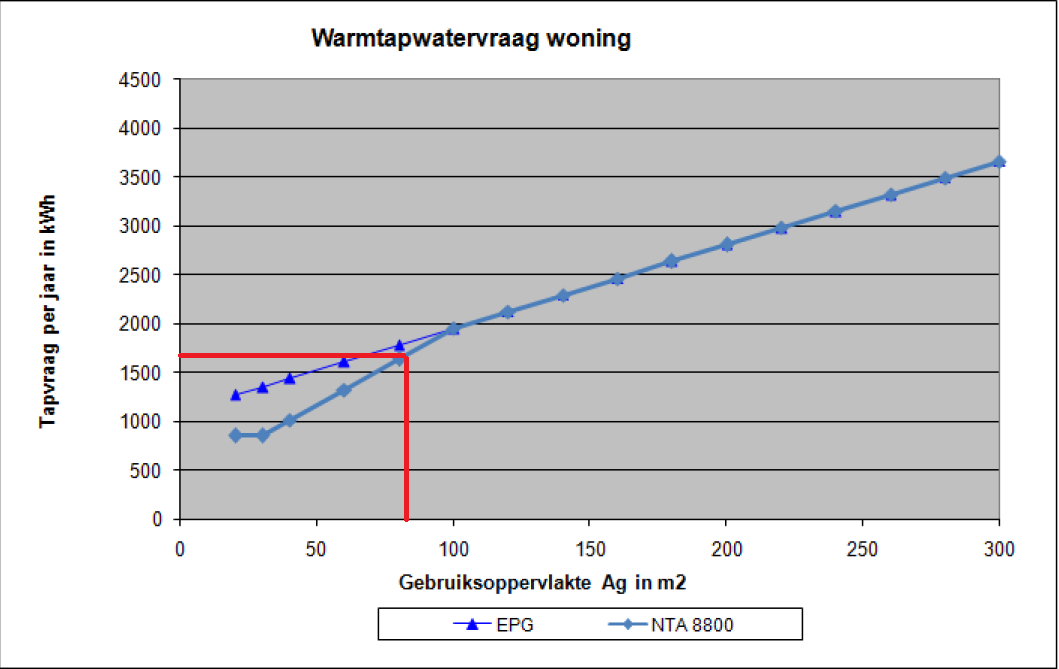
\includegraphics[width=1\columnwidth]{pictures/Tap_water_perm2.png}
% \caption[Short title]{Energy Consumption of the Apartment}
% \label{fig:ff6}\end{figure}.



% An average energy use for heating is 5907.875 kwh per apartment. The heat demand profile for apartment building will be calculated follow equation (2) and (3). 

% \begin{figure}[H]
% \centering
% 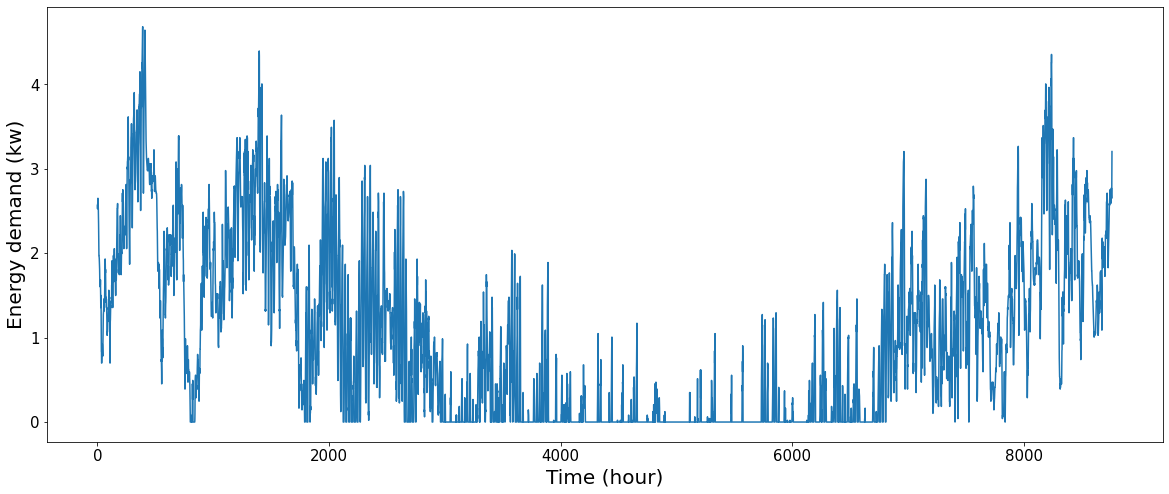
\includegraphics[width=1\columnwidth]{pictures/Apartment_profile.png}
% \caption[Short title]{Energy Consumption of the Apartment.}
% \label{fig:ff6}\end{figure}


\subsection{Hot tap water profile}
 
 
We will analyze a normal Dutch house using CW label 3 or 4 (Appendix A). Therefor,e capacity profile M will be selected as a reference.\\
Capacity profile definition:
Annex III of the EU regulation[3] describes a capacity profile for a 24-hour measurement cycle intended for checking compliance with the requirements.\\
This capacity profile is as follows:

\begin{itemize}
      \item No hot water consumption from 9:35 PM to 7 AM.
      \item From 07:00 to 21:30 hot water consumption according to a precisely defined tap profile.
    \end{itemize}
An example calculation is shown below: 

\begin{figure}[H]
\centering
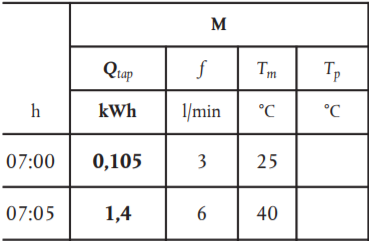
\includegraphics[width=0.6\columnwidth]{pictures/Tap_water example.png}
\caption[Short title]{Tap water example \cite{VERORDENING}.}
\label{fig:twexample}
\end{figure}
At 7.00 $Q_{tap}$ is 0.105 kwh with the flow rate at 3 liters  per minutes and temperature added is 25 degree.

\[m = \frac{3600.Q}{c.\Delta T}\]

m = 6 liters(kg), c=4.19 kj/kg.K. Therefore 2 minutes of tap water has been used at 7.00 AM

The hot tap water profile M for 1 day is showing in figure 10:

\begin{figure}[H]
\centering
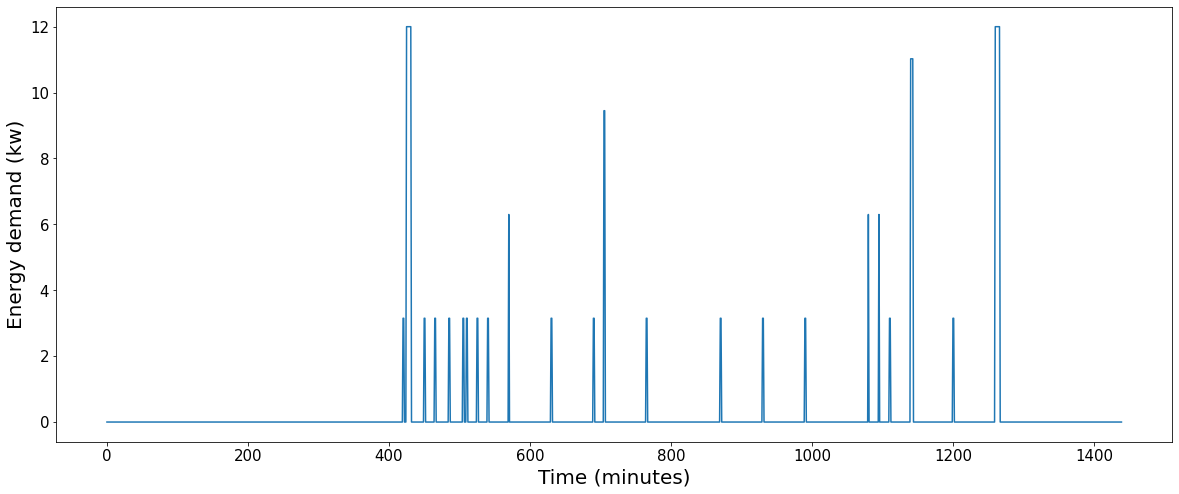
\includegraphics[width=1\columnwidth]{pictures/hot_tap_water_profile_M.png}
\caption[Short title]{hot tap water profile M.}
\label{fig:htwM}
\end{figure}

\subsection{Simulation profile for the entire building}

The simulation is base on the assumption of the apartment building with 24 residential apartments.
The hot tap water demand for 24 apartments will be calculated base on the calculation rules public in kennisbank isso 55.

\begin{figure}[H]
\centering
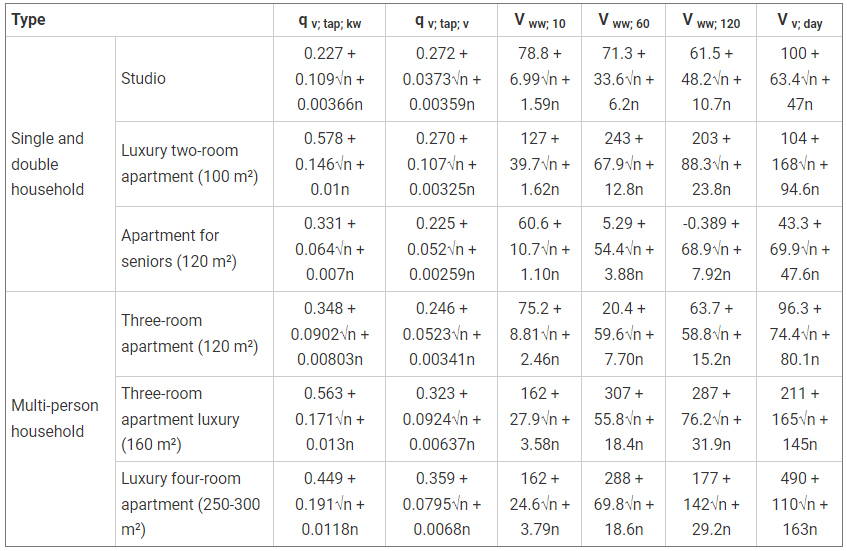
\includegraphics[width=1\columnwidth]{pictures/Calculation rules for hot tap water demand for apartment buildings.png}
\caption[Short title]{Calculation rules for hot tap water demand for apartment buildings[ \cite{ISSO55}.}
\label{fig:calcrules_ap}
\end{figure}
The instantaneous hot water requirement for an hour is:

\begin{figure}[H]
\centering
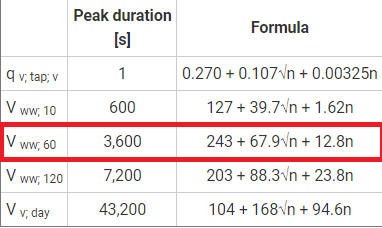
\includegraphics[width=0.5\columnwidth]{pictures/tap water demand in an hour.png}
\caption[Short title]{Calculation rules for hot tap water demand for an hour \cite{ISSO55}.}
\label{fig:calchour}
\end{figure}

\begin{equation}
V_{WW;60} = 243 + 67.9\sqrt{n} + 12.8n
\end{equation}

$V_{WW;60}$: volume flow of hot water in 60 minutes

$n$: number of apartments

The hot tap water profile for a building apartment is shown below:


%Example of the multicolumn command
\begin{table}[h!]
\centering
\begin{tabular}{|p{3cm}|p{3cm}|}
\hline
\multicolumn{2}{|c|}{1 day hot tap water usage} \\
\hline
Time& $Q_{tap}$ (kwh)\\ % & Use periods(hour)
 \hline
 07:00	& 38.64   \\ % &1.1
 08:00  & 10.08   \\ % &0.8
 09:00	& 5.04    \\ % &0.4
 10:00  & 2.52    \\ % &0.1
 11:00  & 5.04    \\ % &0.4
 12:00  & 7.56    \\ % &0.2
 13:00  & 0         \\ %&0
 14:00  & 2.52   \\ %& 0.2
 15:00  & 2.52   \\ % & 0.2
 16:00  & 2.52   \\ % & 0.2
 17:00  & 0        \\ % & 0
 18:00  & 7.56   \\ % & 0.4
 19:00  & 2.52  \\ %  & 0.2
 20:00  & 17.64 7\\ % & 0.3
 21:00  & 36.12 \\ %  & 0.9
 22:00  & 0        \\ % & 0

  \hline
 \end{tabular}
 \caption{Hot water profile}

 \end{table}


\begin{figure}[H]
\centering
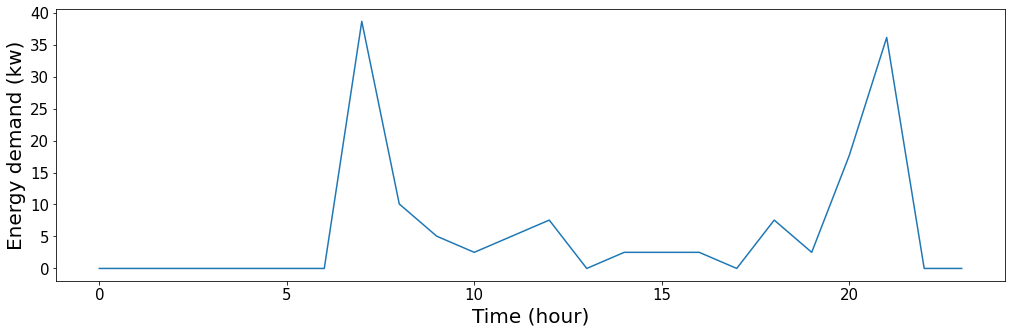
\includegraphics[width=1\columnwidth]{pictures/tap water profile of 24 apartments.png}
\caption[Short title]{Hot tap water use of entire apartment.}
\label{fig:htw_entire}
\end{figure}

% The heat demand for the building:

% \begin{equation}
% Q_{building} = Q_{hotwater} + Q_{heating}
% \end{equation}

% \begin{figure}[H]
% \centering
% 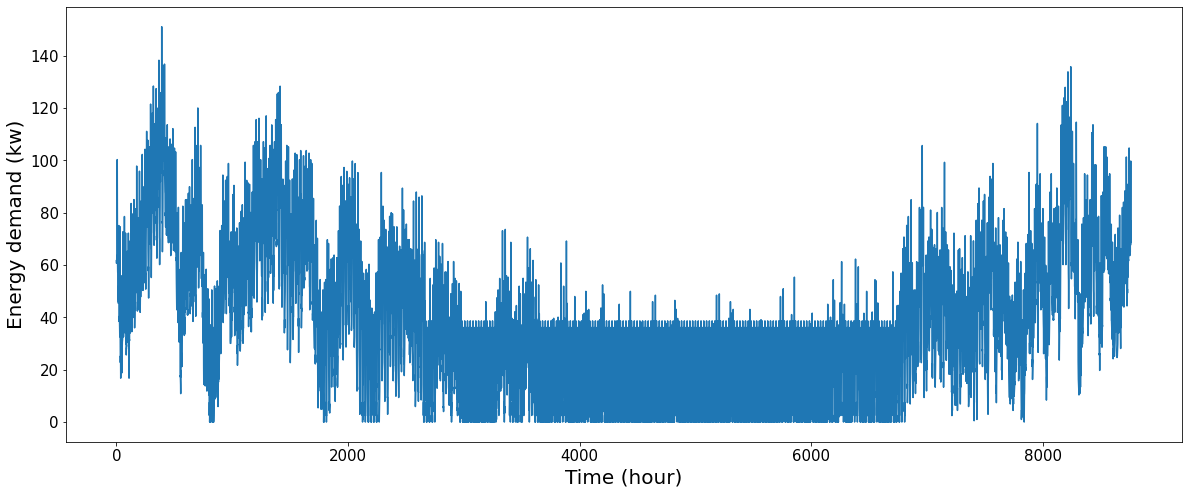
\includegraphics[width=1\columnwidth]{pictures/Q_building profile.png}
% \caption[Short title]{Energy demand for an Apartment.}
% \label{fig:ff12}\end{figure}

\subsection{BENG and load profile correction}

Total energy consumption for D.H.W with profile M \cite{VERORDENING} (Appendix A) is 5,845 kwh per day. The annual consumption is therefore approximately 2134 kwh. The value is much higher than the indicated value ( approximately 1600 kwh) for 77m2 apartments from NTA8800 \cite{NTA8800}, Figure \ref{fig:htwyear}.

\begin{figure}[H]
\centering
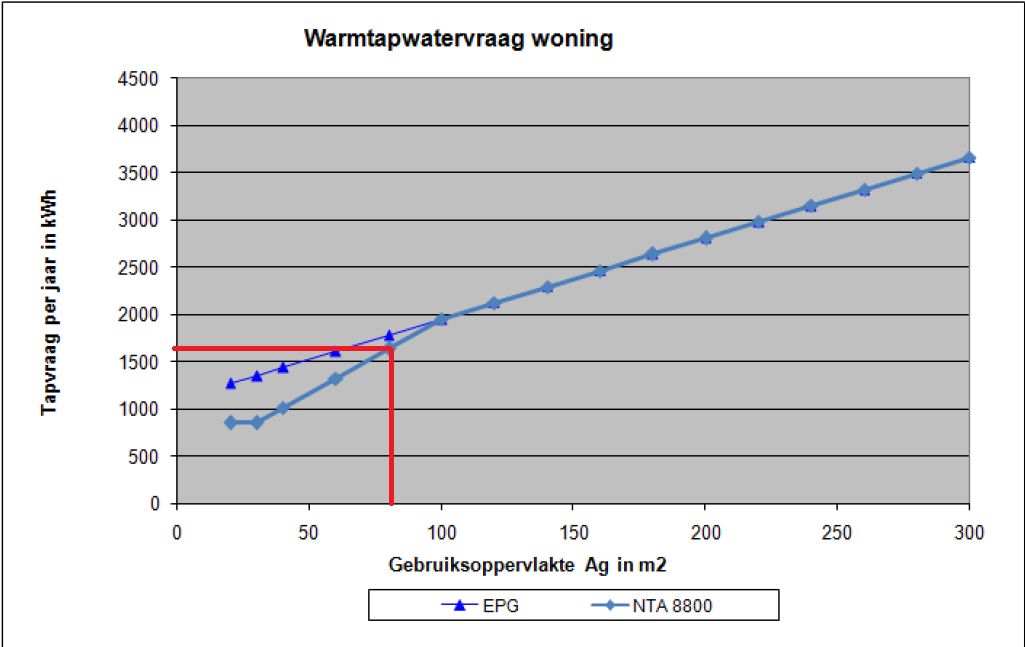
\includegraphics[width=1\columnwidth]{pictures/NTA_8800_DHW.png}
\caption[Short title]{Hot tap water use per year (kwh/$m^2$) \cite{NTA8800}.}
\label{fig:htwyear}
\end{figure}

According to NEN 12831-3 \cite{NEN12831}, Method for calculation of the design heat load - Part 3:  Domestic hot water systems heat load and characterisation of needs. The value of volume of hot water per day ($V_{W;P;day}$) can be calculated based on the number of equivalent persons (adults) $n_{P,eq}$.
\vspace{2mm}
\\
\textbf{Apartment dwellings}.\\
The area is used to calculate $n_{P,eq}$,max as follow: 
\begin{equation}
    n_{P,eq,max}= 1.75 - \begin{cases}
			1, & \text{if $A_{h} < 10 m^2$}\\
            0.01875\cdot(50 - A_h), & \text{if $10 m^2 <A_{h} < 50 m^2$}\\
            0.035\cdot A_h, & \text{if $A_{h} > 50 m^2$}
		 \end{cases}
\end{equation}\\
The total number of equivalent persons is defined by formula:


\begin{equation}
    n_{P,eq}= 1.75 + \begin{cases}
			0.3\cdot n_{P,eq,max}, & \text{if $n_{P,eq,max} < 1.75$}\\
            0.3\cdot(n_{P,eq,max}- 1.75), & \text{if $n_{P,eq,max} \geq 1.75$}
		 \end{cases}
\end{equation}\\
For the residential case and at the level of one dwelling, requirements can be expressed by formula:


\begin{equation}
   V_{W,P,day} = min\Big(x;\Big(y\cdot \frac{A_h}{n_{P,eq}}\Big)\Big)
\end{equation}\\
Where:\\ 
$A_{h}$: habitable area.\\
$n_{P},e_{q}$: number of equivalent persons used for calculating the D.H.W requirements.\\
$n_{P},e_{q,max}$: maximum number of equivalent persons corresponding to the part of the group supplied by the same D.H.W transmitter (individual or attached house and collective housing).\\
The default values for x, and y are:
x = 40,71
y = 3,26 \cite{NEN12831}

Applied equations (13) and (14) for the 77 $m^2$ apartment dwelling.$n_{P},e_{q}$ = 1.4665.

Compare the assumption of define cases with 2.8 people in 77 $m^2$ there are more likely that the EU-M capacity profile was define for more than 1.4 people,


Check--------------------------------------

According to NEN NTA2020 - 13.3.2.1 / 856kwh/jaar/person = 856*2.8= 2396.8

